\documentclass[10pt,a4paper]{article}
\usepackage[utf8]{inputenc}
\usepackage[english]{babel}
\usepackage{amsmath}
\usepackage{amsfonts}
\usepackage{amssymb}
\usepackage{graphicx}
%\usepackage[left=3cm,right=3cm,top=3cm,bottom=3cm]{geometry}

\usepackage{natbib}

\author{Fabian Schubert, Claudius Gros}
\title{Applying a Reduced Model of Apical and Basal Dendritic Compartments to Sequence Learning in Recurrent Neural Networks}
\begin{document}
\maketitle

Experiments suggest that, depending on the amount of apical (distal) and basal dendritic synaptic drive, layer 5 pyramidal neurons can exhibit quietness, low frequency spiking and high frequency bursting \cite{Letzkus_2006,Shai_2015}. The latter only occurs when distal and basal inputs coincide in time. A simplified, rate based compartment model of this effect has been used to gate plasticity of basal connections by means of distal synaptic inputs \cite{Bono_2017}.

We use this mechanism for sequence prediction. In our framework, coincidence detection of distal and basal input modulates plasticity to extract a predictive signal from a recurrent dynamic reservoir. This approach is similar to echo state networks \cite{Jaeger_2010}, but readout and external input are now collected by the same units (see Figure). Combining both streams of information in the previously described manner, the error signal for learning is thus implicitly expressed as the nonlinear response to basal and distal input.

Furthermore, our recurrent reservoir is a self organized balanced network: using a nonlinear Hebbian-type learning rule that is derived from minimizing the fisher information as an objective function \cite{Echeveste_2015}, the network autonomously settles into an inhibitory-excitatory balance, generating rich network dynamics, which is necessary for its use in an echo state framework. 

\begin{figure}
\centering
\includegraphics[width=0.5\textwidth]{illustration.png}
\caption{Architecture of the network}
\end{figure}

\bibliographystyle{unsrt}
\bibliography{sources.bib}

\end{document}